\section{Média- és feliratfájlok választása}

\begin{figure}[!h]
  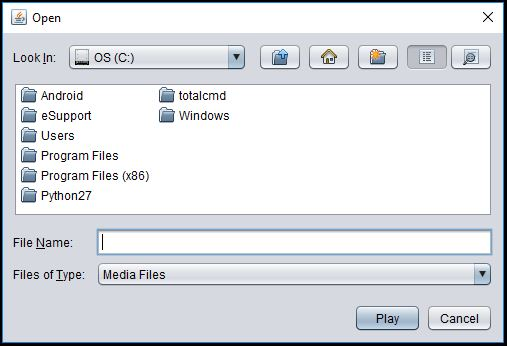
\includegraphics[width=\linewidth]{images/chooser_screen.jpg}
  \caption{Médiafájl választó}
  \label{fig:chooser_screen}
\end{figure}

A médiafájlok lejátszása a videólejátszó alkalmazás elengedhetetlen részét képezik, hiszen enélkül a felhasználó képtelen lenne, vagy csak komplikált módszerek igénybevételével tudná megtekinteni videó fájljait. A feliratok megjelenítése a szoftver egy másik sarkallatos pontja. E funkció teszi lehetővé a felhasználó számára, hogy filmjeit idegennyelven feliratozva tekinthesse meg. Mindkettő megvalósítása egy tallózó segítségével történik, amely a megszokott módon, gyorsan, kényelmesen enged utat a fájlválasztásnak. Alapesetben a választó a felhasználó \textit{home} könyvtárában nyílik, onnan navigálva kereshetők a tartalmak. A fájlok kiválasztása után azok azonnal megjelennek a képernyőn, valamint videó fájlok esetén el is indulnak. A tallózók megvalósítása \textit{Java Swing} komponensek, azon belül \textit{JButton}, \textit{JFileChooser} segítségével történtek. A médiafájl választás folyamata a \textit{Load/Eject media} gomb megnyomásával indítható el, amely a vezérlőpanel jobb alsó részén elérhető, és a \ref{fig:chooser_screen}-es ábrán látható ablakot jeleníti meg. A gombhoz használt ikont a \textit{resources/icons} könyvtárból importáltam. A fájlválasztáshoz a könnyebb használat érdekében szűrőket definiáltam, amelyek a fájlok kiterjesztése alapján szűrik meg az éppen aktuális könyvtár tartalmát, és jelenítik meg csak azokat az elemeket, amelyek a feltételnek megfelelnek. Ezek külön-külön a videó, audió, lejátszási lista, illetve a médiafájlokra való szűrést teszik lehetővé. Ezeken felül elérhető egy \textit{All files} opció is, amely filterezés nélkül az összes elérhető fájlt kilistázza a felhasználó számára. Ezen szűrőket a fájlválasztó \textit{Files of Type} címke mellett található legördülő listából választhatjuk ki. Amennyiben ennél specifikusabb módon szeretnénk keresni, lehetőségünk van a keresőmező használatára. Ezt a \textit{File Name} felirat mellett található mezőbe írt kulcsszavak segítségével tehetjük meg. Ha gyorsabban szeretnénk navigálni a könyvtárak között, ezt megtehetjük a választó felső részén fellelhető legördülő listából kiválasztható elemekkel. Itt megtalálhatók a számítógépen elérhető fő könyvtárak, mint például a különböző meghajtók, asztal és egyéb nagyobb méretű mappák. A lista helyzetétől jobbra felfedezhető néhány további gomb. Ezek rendre: egy szinttel feljebb lépés a könyvtárhierarchiában, vissza a \textit{home} könyvtárba, új mappa létrehozása, lista- illetve részletes nézet közötti váltás. Ha megtaláltuk az általunk lejátszani kívánt fájlt, kijelölés után a \textit{Play} gomb megnyomásával, illetve a fájlon történő dupla kattintással indíthatjuk el azt. Ugyanezen komponens használatával valósítottam meg a feliratfájlok kiválasztásának kezelését is. Az ablakot a kezelőpanelen fellelhető \textit{Select subtitle} gombra történő kattintással jeleníthetjük meg. A különbség csupán annyi a két ablak között, hogy a feliratfájl-választó ablakban más szűrők definiáltak. Ez értelemszerűen a feliratfájlok kizárólagos megjelenítésére ad lehetőséget. Mindkét ablak esetében kényelmi funkcióként implementálásra került az elérési útvonal megjegyzése. Amikor a felhasználó fájlt választ, legyen a média, vagy felirat, az alkalmazás elmenti a fájl elérési útvonalát, és ez alapján állítja a tallózó az aktuális kiinduló könyvtárát.

\begin{spacing}{1.25}
\begin{lstlisting}[caption=Aktuális könyvtár beállítása, label={lst:aktualis_konyvtar}, language=java]
	if(actualFile != null)
	    {fileChooser.setCurrentDirectory(actualFile);
	}
\end{lstlisting}
\end{spacing}
        
A \ref{lst:aktualis_konyvtar}-es kódrészlet néhány sorában mindösszesen annyi történik, hogy amennyiben az aktuális fájl, azaz az utolsóként kiválasztott fájl nem üres, akkor a tallózó aktuális könyvtára a fájlt tartalmazó mappa lesz. Ugyanez a kódrészlet megtalálható a feliratfájl választó kódjában is. Mindezeken felül a fájlválasztó másik módon is megjeleníthető. A felső menüsávban a \textit{Media} menüpont alatt található \textit{Play Media…} menü kiválasztásával a tallózó megjelenik a képernyőn. Itt akár gyorsbillentyűvel, úgynevezett mnemonikkal is hatékonyabbá tehetjük a fájlválasztást elindítását. A menüsávban található \textit{Media} az \textit{"m"}, a \textit{Play File…} menü pedig az \textit{"f"} billentyűk lenyomásával hívható elő.
 Az implementált két tallózó a fent említett részletek alapján alkalmas fájlok gyors és hatékony szelekciójára, olyan módon, hogy azt egy átlagfelhasználó is könnyedén, kevés kutatással megteheti.
